\subsection{Part Selection}
\noindent For \textbf{obstacle detection}, the final selections are:
\begin{enumerate}
	\item 2x HC-SR04 Multistatic Ultrasonic Sensors for lateral-facing detection.
	\item 2x RCWL-1005 Monostatic Ultrasonic Sensors for front-facing detection.
	\item The TFLuna LiDAR sensor, for its precision and accuracy. Front-facing. It has easy I2C configuration and a great price point, making it a viable option.
	\item The BNO-055 Inertial Measurement Unit because of its advantages like quaternion output and affordability, which greatly enhance FORWARD stability.
\end{enumerate}

\noindent For \textbf{obstacle identification}, the final selections are:
\begin{enumerate}
	\item The ESP32 MCU for affordability and diverse I/O ports. 
	\item The Realtek AMB82-Mini IoT AI Camera for high performance, cost-effectiveness, high image quality.
	\begin{enumerate}
		\item A stretch requirement of our project is to implement a depth perception capability with our system. Due to the sensor fusion solution that we are taking we have decided that we no longer need a super high-quality camera to obtain the depth data.
	\end{enumerate}
	\item The YOLO model family for memory size flexibility and user-friendly libraries for simple integration.
	\item The YouthWhisper Bone Conduction headphones for affordability and battery life.
\end{enumerate}


\noindent For \textbf{obstacle avoidance}, the final selections are:
\begin{table}[H]
	\centering
	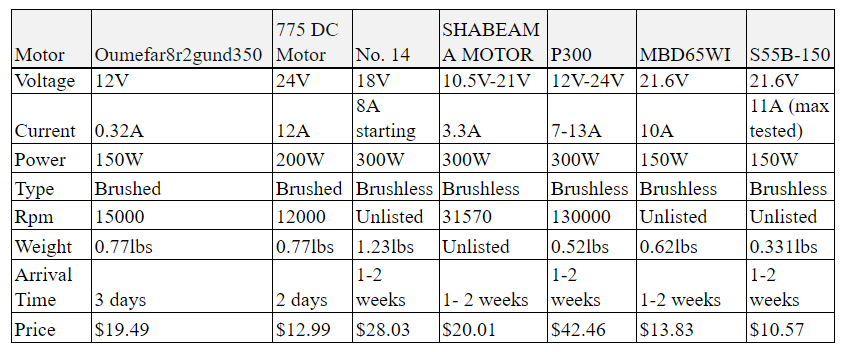
\includegraphics[width=1\textwidth]{./Images/drive_motors.png}
	\caption{\label{fig:drive_motors}Drive Motor Specifications}
\end{table}


\noindent When deciding on what DC motors that we wanted to use, our main concerns were power, current rating, motor type, and price. It was calculated that in order to meet the speed requirements, we needed a total of 300W or 150W per motor. All of the motors investigated thus are at least 150W. It was also preferable to use brushless DC motors, as they are higher in quality (longevity, efficiency, low noise) than brushed DC motors and are more widely compatible with motor drivers. To decide between the brushless DC motors, we mostly looked at price and found the most cost-effective motors, while also keeping in mind the current rating so that we can purchase motor drivers with a large enough current rating to supply the motors. Thus, we decided to use the S55B-150 DC motors. \cite{yzl1} \cite{Citphto} \cite{AliExpress1} \cite{AliExpress2} \cite{AliExpress3} \cite{PrecisionMicrodrives} \cite {AliExpress8}\\

\begin{table}[H]
	\centering
	\setlength{\tabcolsep}{5pt} % Restore default column padding
	\renewcommand{\arraystretch}{1.75} % Restore default row height
	\scalebox{0.85}{ % Scale down the entire table by 75%
		\begin{NiceTabular}{|l|c|c|c|}[hvlines,colortbl-like]
			\CodeBefore
			\rowcolor{gray!15}{1}
			\Body
			\textbf{Specification} & \textbf{B0B4SK8M1C \cite{DIANN}} & \textbf{A19090500ux0371 \cite{uxcell}} & \textbf{Vibration Motor \cite{eBayDC}} \\ 
			\hline 
			Voltage & 1.5-3.7V & 4.5-12V & 3-5V \\ 
			\hline 
			Current & 85mA & 250mA & 15mA \\ 
			\hline 
			Type & DC & DC & DC \\ 
			\hline 
			Arrival Time & 4 days & 4 days & 1-3 weeks \\ 
			\hline 
			Price (Qty) & \$5.99 (10) & \$10.99 (2) & \$9.21 (2) \\ 
		\end{NiceTabular}
	}
	\caption{\label{fig:vibrationMotorSpecifications}Vibration Motor Specifications}
\end{table}

\noindent Haptic motors are small DC motors that are used for vibration feedback in the handlebars of the walker. Because they are only used for the purpose of vibration, these motors are very small and do not draw much current. Our main concern with deciding which haptic motors to use is the voltage rating and price. In order to be compatible with most motor drivers, the motors should be able to be operated at both 5V and 3V. Although not the most cost-effective, we chose the "Vibration Motor" as it has the largest compatibility with motor drivers.\\

\begin{table}[H]
	\centering
	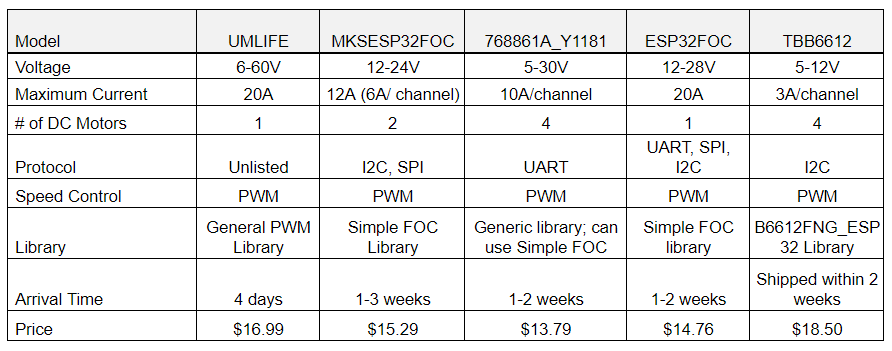
\includegraphics[width=1\textwidth]{./Images/motor_controller_table2.png}
	\caption{\label{fig:motor_controller}Motor Controller Specifications}
\end{table}

\noindent After comparing multiple factors, we ultimately chose the 768861A\_Y1181 motor controller. This is because our main concern was supplying current to the motors and operating all 4 motors from the same controller. The motors that we chose to drive the wheels draw up to 11A of current, which the 768861A\_Y1181 would be able to handle, although it is rated for 10A, upon examining the data sheet. This motor controller also provides a wide voltage range of 5-30V, which is able to provide the correct voltage for both the wheel-driving motors and the haptic motors. The 768861A\_Y1181 also happens to be the most cost-effective of the motor controllers. \cite{UMLIFE} \cite{AliExpress5} \cite{Makerbase} \cite{AliExpress7} \cite{CircuitBasics} \cite{Espressif1} \cite{AliExpress4} \cite{Burgess} \cite{RandomNerd} \cite{Espressif2} \cite{SimpleFOC} \cite{SimpleFOC2} \cite{Peza}\\


\begin{table}[H]
	\centering
	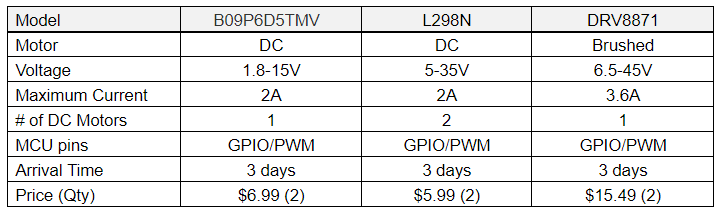
\includegraphics[width=1\textwidth]{./Images/haptic_driver_table_2.png}
	\caption{\label{fig:haptic_driver}Haptic Motor Driver Specifications}
\end{table}

\noindent This table compares the different motor drivers available for use with haptic motors.  decided to use the L298N motor driver as this solution is simply the most cost-effective. All of the haptic motor driver options available have similar ratings in voltage and current. We were also able to find more documentation for the L298N \cite{BOJACK} \cite{BEEYDC} \cite{HiLetgo}.\\

\begin{table}[H]
	\centering
	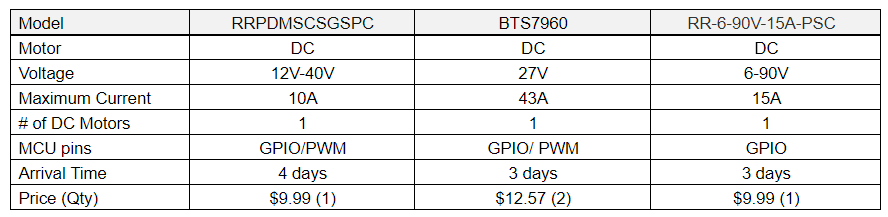
\includegraphics[width=1\textwidth]{./Images/wheel_driver_table.png}
	\caption{\label{fig:wheel_driver}Wheel Motor Driver Specifications}
\end{table}

\noindent Comparing options, we decided upon using the BTS7960 motor driver. The BTS7960 is able to supply more than enough current to the DC motors driving the wheels. This option is also the most cost-effective as the price includes two motor drivers to be able to drive both motors \cite{RioRand} \cite{Gikfun} \cite{Hobbywing}.\\

\begin{table}[H]
	\centering
	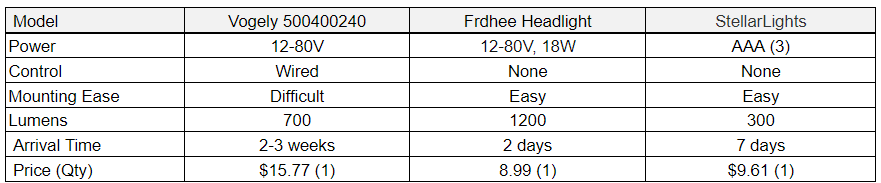
\includegraphics[width=1\textwidth]{./Images/headlight_table.png}
	\caption{\label{fig:headlights}Comparison of Headlight Options}
\end{table}

\noindent Comparing these different headlights that were originally intended for bicycles and motorcycles, we decided to use the Vogely ‎500400240. This is because these are the only headlights of these options that are able to be controlled digitally. Headlights are only necessary in dark environments, so we must connect the headlights to a light sensor. \cite{vogely2024} \cite{frdhee2024} \cite{stellarlights2024}\\

\begin{table}[H]
	\centering
	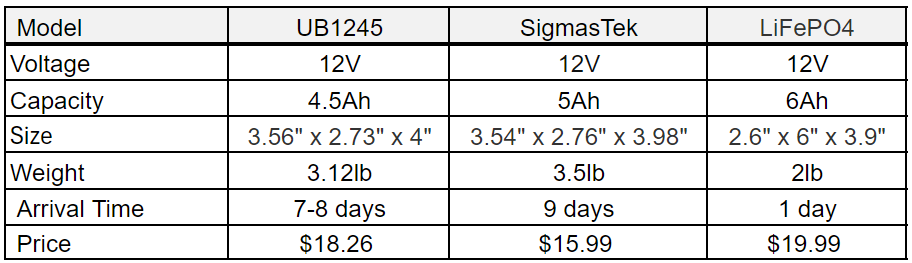
\includegraphics[width=1\textwidth]{./Images/battery_table.png}
	\caption{\label{fig:batteries}Comparison of Battery Options}
\end{table}

\noindent Comparing these different options for batteries, we decided upon using the SigmasTek battery. We evaluated 12V batteries since we ultimately decided on implementing 12V motors and these are our highest-voltage components. Comparing prices and capacity, we found that the SigmasTek battery was preferred because it provides the lowest cost for the needed battery capacity. \cite{liftmaster2024} \cite{lifepo42024} \cite{ub12452024}\\